\documentclass{article}
\usepackage{amsmath, amssymb, tikz, geometry, graphicx, natbib, mwe, xcolor,
 listings, tabularx, pdfpages, blindtext, mathtools, stackengine, amsthm, pgfplots,bigints, relsize, upgreek, esint, array, multirow, schemata}
\usepackage{hyperref}
\usepackage{slashed, enumitem}


\pgfplotsset{width=10cm,compat=1.9}

\colorlet{myWhite}{white!35!gray}
\definecolor{shadeofgray}{HTML}{181818}
\definecolor{shadeofviolet}{HTML}{0f022c}



\hypersetup{
    colorlinks=true,
    linkcolor=violet,
    filecolor=magenta,      
    urlcolor=cyan,
    pdftitle={Overleaf Example},
    pdfpagemode=FullScreen,
}

\geometry{ 
 a4paper,
 total={170mm,257mm},
 left=20mm,
 top=10mm,
 }
 
\lstdefinestyle{mystyle}{ 
bracketsstyle=\color{red}
}

\title{Economia e Organizzazione Aziendale}
\author{Giuseppe Bumma}


%----------------------------------------------------------------------
%use this for a total black background
%\pagecolor{black}
%\color{myWhite}
%----------------------------------------------------------------------


\pagecolor{shadeofgray}
\color{myWhite}



\begin{document}

%Commands
\newcommand{\R}{\mathbb{R}}
\newcommand{\bb}[1]{\mathbb{#1}}
\newcommand{\cc}[1]{\mathcal{#1}}
\newcommand{ \lognormal }{\text{Lognormal} }
\newcommand{\tb}[1]{\textbf{#1}}
\newcommand*\circled[1]{\tikz[baseline=(char.base)]{%
            \node[shape=circle,draw,inner sep=2pt] (char) {#1};}}
%for using circled number in enumerate use:
%\begin{enumerate}[label=\protect\circled{\arabic*}]


\tableofcontents

\maketitle

\section{Introduzione alla contabilità}
\subsection{Cos'è un'azienda}
L'azienda è una organizzazione costituita da persone e da beni che, attraverso
una serie coordinata di operazioni, mira alla produzione e allo scambio di beni o
di servizi per soddisfare un bisogno.
\begin{itemize}
    \item \textbf{Definizione giuridica:} il codice civile (art. 2555) definisce azienda il complesso di beni
    organizzati da un soggetto (l'imprenditore), strutturato funzionalmente per
    l'esercizio dell'impresa (produzione di beni e servizi);
    \item \textbf{Definizione "economica":} istituto economico duraturo volto alla produzione di
    beni/servizi, per il soddisfacimento (diretto o indiretto) dei bisogni umani.
\end{itemize}


\subsubsection{Economia aziendale}
L'economia aziendale studia il ciclo
di vita e le condizioni di equilibrio
dell'azienda attraverso l'osservazione
dei fenomeni economici delle
aziende singole e dei loro aggregati; il \textit{sistema azienda} produce beni
per soddisfare i bisogni umani ed è
volto alla realizzazione degli obiettivi
del soggetto economico.
\vspace*{0.2cm}\\
Aspetti fondanti della gestione aziendale sono:
\begin{itemize}
    \item l'organizzazione aziendale;
    \item la gestione;
    \item la rilevazione e il controllo, attraverso l'analisi di \textbf{contabilità} e il controllo di gestione.
\end{itemize}



\subsection{La contabilità}
La Contabilità ha il fine di supportare
l'attività decisionale di chi governa
l'impresa e di tutti coloro che sono
interessati a conoscere le sue condizioni
economiche, finanziarie, patrimoniali. Sostanzialmente è il
processo di raccolta, misurazione, analisi,
interpretazione e comunicazione di
informazioni economiche e finanziarie che
consentano ai decisori di esprimere giudizi
e valutazioni sull'impresa.\\
Le informazioni sono necessarie agli \textit{shareholders}(azionisti, che sono effettivamente soci) e agli \textit{stakeholders} (coloro che hanno contatti con l'azienda, come clienti o fornitori)
\vspace*{0.1cm}\\
La contabilità ha le
seguenti caratteristiche: 
\begin{itemize}
    \item ha natura \textbf{tecnica}
    \item è guidata da regole;
    \item evolve in risposta ai cambiamenti
    economici e sociali.
\end{itemize}


\subsubsection{I concetti alla base
della contabilità}
I concetti o principi sono regole generali
che guidano l'azione, ma non prescrivono
esattamente come si debba registrare un
evento.
\vspace*{0.1cm}\\
I criteri alla base della formulazione dei
principi sono:
\begin{itemize}
	\item Rilevanza (di solito i costi di produzione)
    \item Oggettività
    \item Fattibilità
\end{itemize}
\noindent\fbox{%
\parbox{\linewidth}{%
\centering Il fine ultimo del processo contabile è la
produzione di \textbf{rendiconti economico-finanziari} \newline che sintetizzano il risulto della
gestione.
}%
}
\begin{center}
    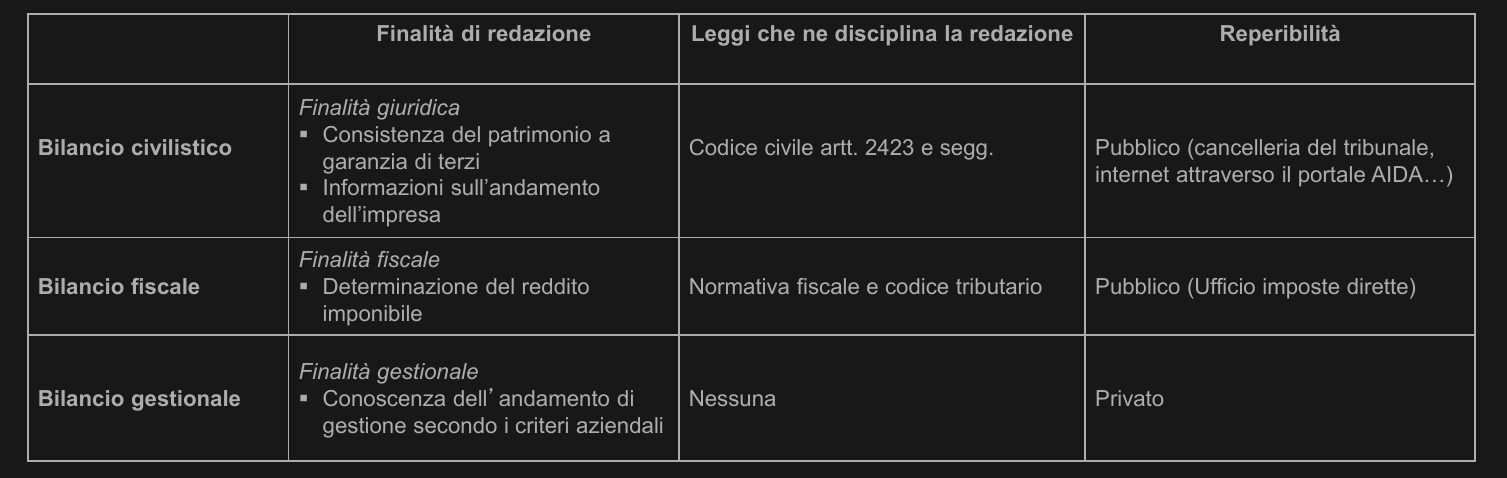
\includegraphics[scale=0.4]{Tabella bilancio.png}
\end{center}
\textbf{N.B.} Il bilancio fiscale si chiude sempre a dicembre, ma un'azienda può compilare un bilancio gestionale (con cadenza arbitraria, as es. mensile o bimestrale) per avere un'idea sui futuri investimenti.


\subsubsection*{I soggetti economici interessati al bilancio}
\begin{itemize}
    \item Portatori interessi
    della comunità locale e
    nazionale
    \item Management e organi di governo
    \item Lavoratori dipendenti
    \item Lavoratori in cerca d'impiego
    \item Banche
    \item Fornitori
    \item Erario
    \item CLienti
    \item Concorrenti
    \item Sindacati
\end{itemize}


\section{I rendiconti economico-finanziari}
\subsection{Bilancio}
Il \textbf{bilancio} è  composto di 4 documenti
principali:
\begin{itemize}
    \item Lo \textbf{Stato Patrimoniale}
    \item Il \textbf{Conto Economico}
    \item Il \textbf{Rendiconto dei flussi di cassa}
    \item La \textbf{Nota Integrativa} (che noi non tratteremo)
\end{itemize}

\subsubsection{Lo stato Patrimoniale}
Lo Stato Patrimoniale rappresenta un'\textbf{istantanea}
della posizione patrimoniale e finanziaria di
un'azienda, cioè la sua posizione in un dato
momento. Esso fornisce tre informazioni essenziali:
\begin{itemize}
    \item che il rendiconto è uno stato patrimoniale\
    \item il nome dell'azienda al quale il rendiconto si riferisce
    \item la data alla quale il rendiconto si riferisce
\end{itemize}
\textbf{Esempio di un rendiconto:}
\begin{center}
    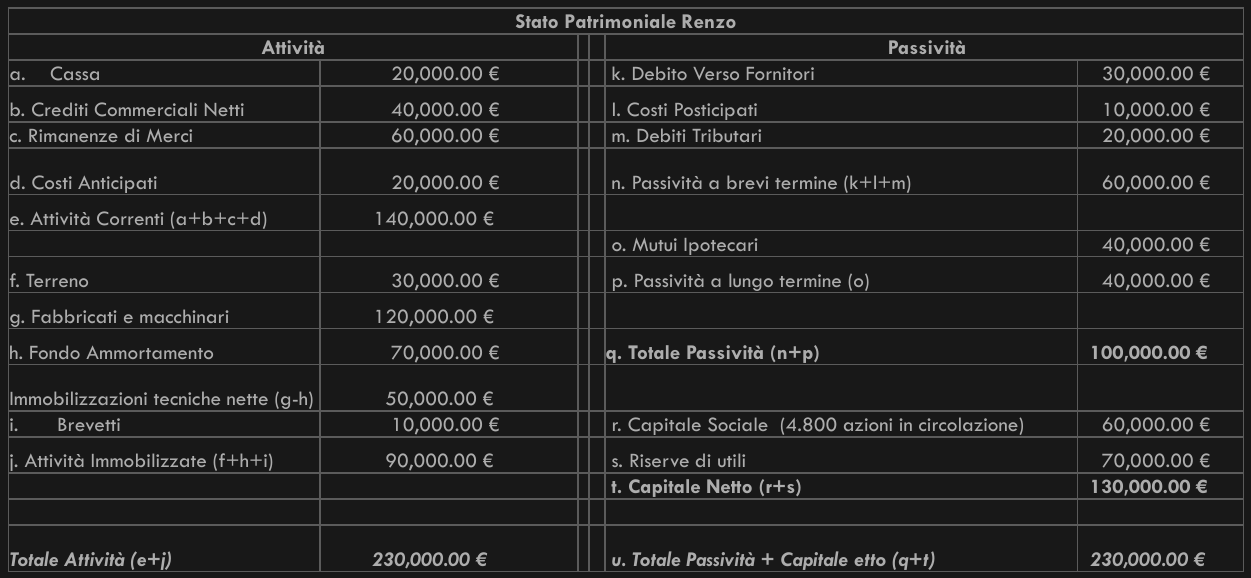
\includegraphics[scale=0.45]{Rendiconto renzo.png
    }
\end{center}
Le \textbf{attività} sono interpretabili come:
\begin{itemize}
    \item Risorse economiche possedute dall'azienda
    \item Impieghi o investimenti aziendali compiuti per perseguire gli obiettivi
aziendali
\end{itemize}
Le \textbf{passività} sono interpretabili come:
\begin{itemize}
    \item Diritti dei creditori nei confronti delle attività aziendali
    \item Obblighi nei confronti dei creditori
    \item Fonti finanziarie messe a disposizione dai creditori
\end{itemize}
Il \textbf{capitale netto} è interpretabile come:
\begin{itemize}
    \item Diritti (residuali) della Proprietà nei confronti delle attività aziendali
    \item Fonti finanziarie messe a disposizione dalla Proprietà
\end{itemize}
L'aumento di capitale netto di un periodo determinato esclusivamente dalle
operazioni di gestione si chiama \textbf{reddito} o \textbf{profitto} o utile (\underline{non} si chiama
guadagno).
\vspace*{0.2cm}\\
Il concetto (formula) da tenere sempre a mente è 
\begin{center}
    ATTIVITÀ = PASSIVITÀ + CAPITALE NETTO
\end{center}



\subsection{Le attività}
\begin{center}
    Le \textbf{attività} sono risorse economiche controllate da un'azienda il cui costo può essere misurato in maniera affidabile al momento dell'acquisizione.
\end{center}
Un'attività deve:
\begin{enumerate}
    \item Essere stata acquisita attraverso una transazione
    \item Essere una risorsa economica
    \item Essere controllata dall'azienda
    \item Il suo costo (o il suo fair value) deve essere misurabile in modo attendibile al momento dell'acquisto
\end{enumerate}
\textbf{N.B.} se un mio pezzo di patrimonio (es. un terreno) subisce una variazione di valore nel tempo questo non viene riportato nello stato patrimoniale.


\subsection{Le attività correnti e le attività
immobilizzate}
\begin{center}
    \renewcommand{\arraystretch}{2}
    \begin{tabular}{|m{5cm}|m{5cm}|}
        \hline 
        \textbf{Attività correnti o attività a breve termine} & \textbf{Attività a lungo termine o immobilizzate}\\
        \hline 
        Attività che si "trasformeranno" in liquidità entro l'esercizio successivo & \multirow{2}{14em}{Immobilizzazioni materiali Immobilizzazioni immateriali  Immobilizzazioni finanziarie}
        \\
        Attività che produrranno la loro utilità entro l'esercizio successivo (di solito l'anno successivo) & \\
        \hline 
    \end{tabular}
\end{center}


\subsubsection{Le attività correnti}
Si definiscono \textbf{correnti} (o a breve termine) le liquidità vere e proprie e,
inoltre, quelle attività che si presume si \textit{trasformeranno} in liquidità entro un anno:
\begin{enumerate}
    \item Liquidità in senso stretto
    \begin{itemize}
        \item Cassa
        \item Conto corrente attivo
    \end{itemize}
    \item Altre attività correnti
    \begin{itemize}
        \item Titoli immediatamente smobilizzabili
        \item Crediti commerciali
        \item Crediti commerciali verso società del gruppo
        \item Crediti finanziari a breve
        \item Rimanenze
    \end{itemize}
\end{enumerate}


\subsubsection{Le attività immobilizzate}
Le attività \textbf{immobilizzate} sono quelle che produrranno la loro utilità su di un arco temporale \underline{pluriennale} o che si
trasformeranno in liquidità in momenti situati \underline{oltre l'esercizio successivo} a quello della data del bilancio.
\begin{enumerate}
    \item Immobilizzazioni \textbf{materiali}
    \begin{itemize}
        \item Terreno
        \item Fabbricati e immobili
        \item Impianti e macchinari
        \item Attrezzature e stampi
        \item Mobili e macchine da ufficio 
    \end{itemize}
    \item Immobilizzazioni \textbf{immateriali}
    \begin{itemize}
        \item Brevetti
        \item Marchi
    \end{itemize}
    \item Immobilizzazioni \textbf{finanziarie} 
    \begin{itemize}
        \item Partecipazioni (strategiche)
        \item Crediti finanziari a lungo termine
    \end{itemize}
\end{enumerate}


\subsubsection{Le immobilizzazioni tecniche}
Sono le immobilizzazioni materiali strumentali allo svolgimento delle operazioni, a esclusione del terreno. Ne sono esempi i fabbricati, i macchinari, gli impianti e le attrezzature, essendo beni intangibili a utilizzo
pluriennale, cioè risorse che si prevede producano la loro utilità su più periodi
amministrativi.
\vspace*{0.2cm}\\
A differenza dei terreni, le immobilizzazioni tecniche hanno vita economica, alla fine della
quale diventano inutilizzabili, ossia non possono più essere considerate un'attività (anche se si continua a utilizzarli).
\vspace*{0.2cm}\\
Il processo di ripartizione del costo d'acquisto di un bene a utilizzo pluriennale tra gli
anni della sua vita utile è denominato \textbf{\color{violet} ammortamento}; al di là della definizione rigorosa, è la percentuale del valore che ogni anno un immobile perde. La vita utile di un'immobilizzazione tecnica è stimata, in genere, da enti preposti, sulla base della quantità di merce prodotta.\\
Alla fine della vita utile, in alcuni casi, le imprese vendono l'immobilizzazione tecnica, denominata \textbf{valore di recupero}.
\begin{center}
    COSTO DA AMMORTIZZARE = COSTO ACQUISTO - VALORE DI RECUPERO
\end{center}


\subsubsection{Le immobilizzazioni immateriali}
\begin{itemize}
    \item CONCESSIONI: diritti attribuiti dalla Pubblica Amministrazione in virtù dei quali l'azienda può: 1. sfruttare beni pubblici quali miniere, suolo demaniale e altro ancora; 2. gestire servizi pubblici in condizioni regolamentate
    \item LICENZE: conferiscono il diritto di: 1. utilizzare a seguito di specifici contratti: software sviluppato da altri; sistemi e procedure commerciali; 2. esercitare un diritto, come per esempio una licenza di gestione di un esercizio pubblico
    \item MARCHI: sono emblemi, denominazioni o segni che caratterizzano i prodotti valorizzando l'immagine dell'azienda sul mercato
    \item BREVETTI: sono diritti in base ai quali le imprese possono impedire ad altri di beneficiare, per un determinato periodo, di un prodotto o di un processo sviluppati con tecnologia originale
    \item AVVIAMENTO: differenza tra il prezzo pagato per l'acquisto di una azienda e il fair value delle attività nette
\end{itemize}


\subsection{Le passività correnti}
\textbf{Passività correnti finanziarie}
\begin{itemize}
    \item Debiti a breve verso banche
    \item Debiti a breve verso società del gruppo
    \item Quote a breve termine di debiti a lungo termine
\end{itemize}
\textbf{Passività correnti operative (di funzionamento)}
\begin{itemize}
    \item Debiti verso fornitori
    \item Cambiali passive commerciali
    \item Debiti tributari
    \item Debiti verso il personale
    \item Costi sospesi
\end{itemize}





\subsection{Le passività a lungo termine}
\begin{itemize}
    \item Prestiti obbligazionari
    \item Mutui (esclusa la quota in scadenza)
    \item Debiti a lungo termine verso società del gruppo
    \item Debiti verso erario a lungo termine
    \item Trattamento di fine rapporto (T.F.R.)
    \item Fondo imposte a lungo termine
\end{itemize}



\subsection{Il capitale netto}
Gli elementi principali costituenti il capitale netto:
\begin{enumerate}
    \item Capitale versato: ammontare di denaro (o beni) apportato direttamente dalla proprietà (azionisti qualora si tratti di una s.p.a.)
    \item Riserve di utili: "ricchezza" generata attraverso la gestione e non distribuita sotto forma di dividendi
\end{enumerate}




































\end{document}